\documentclass[border=10pt]{standalone}

\usepackage{tikz}
\usepackage{tikzsymbols}
\usetikzlibrary{calc,patterns,shapes.geometric}

\def\centerarc[#1](#2)(#3:#4:#5){\draw[#1] ($(#2)+({#5*cos(#3)},{#5*sin(#3)})$) arc (#3:#4:#5);}

\begin{document}
	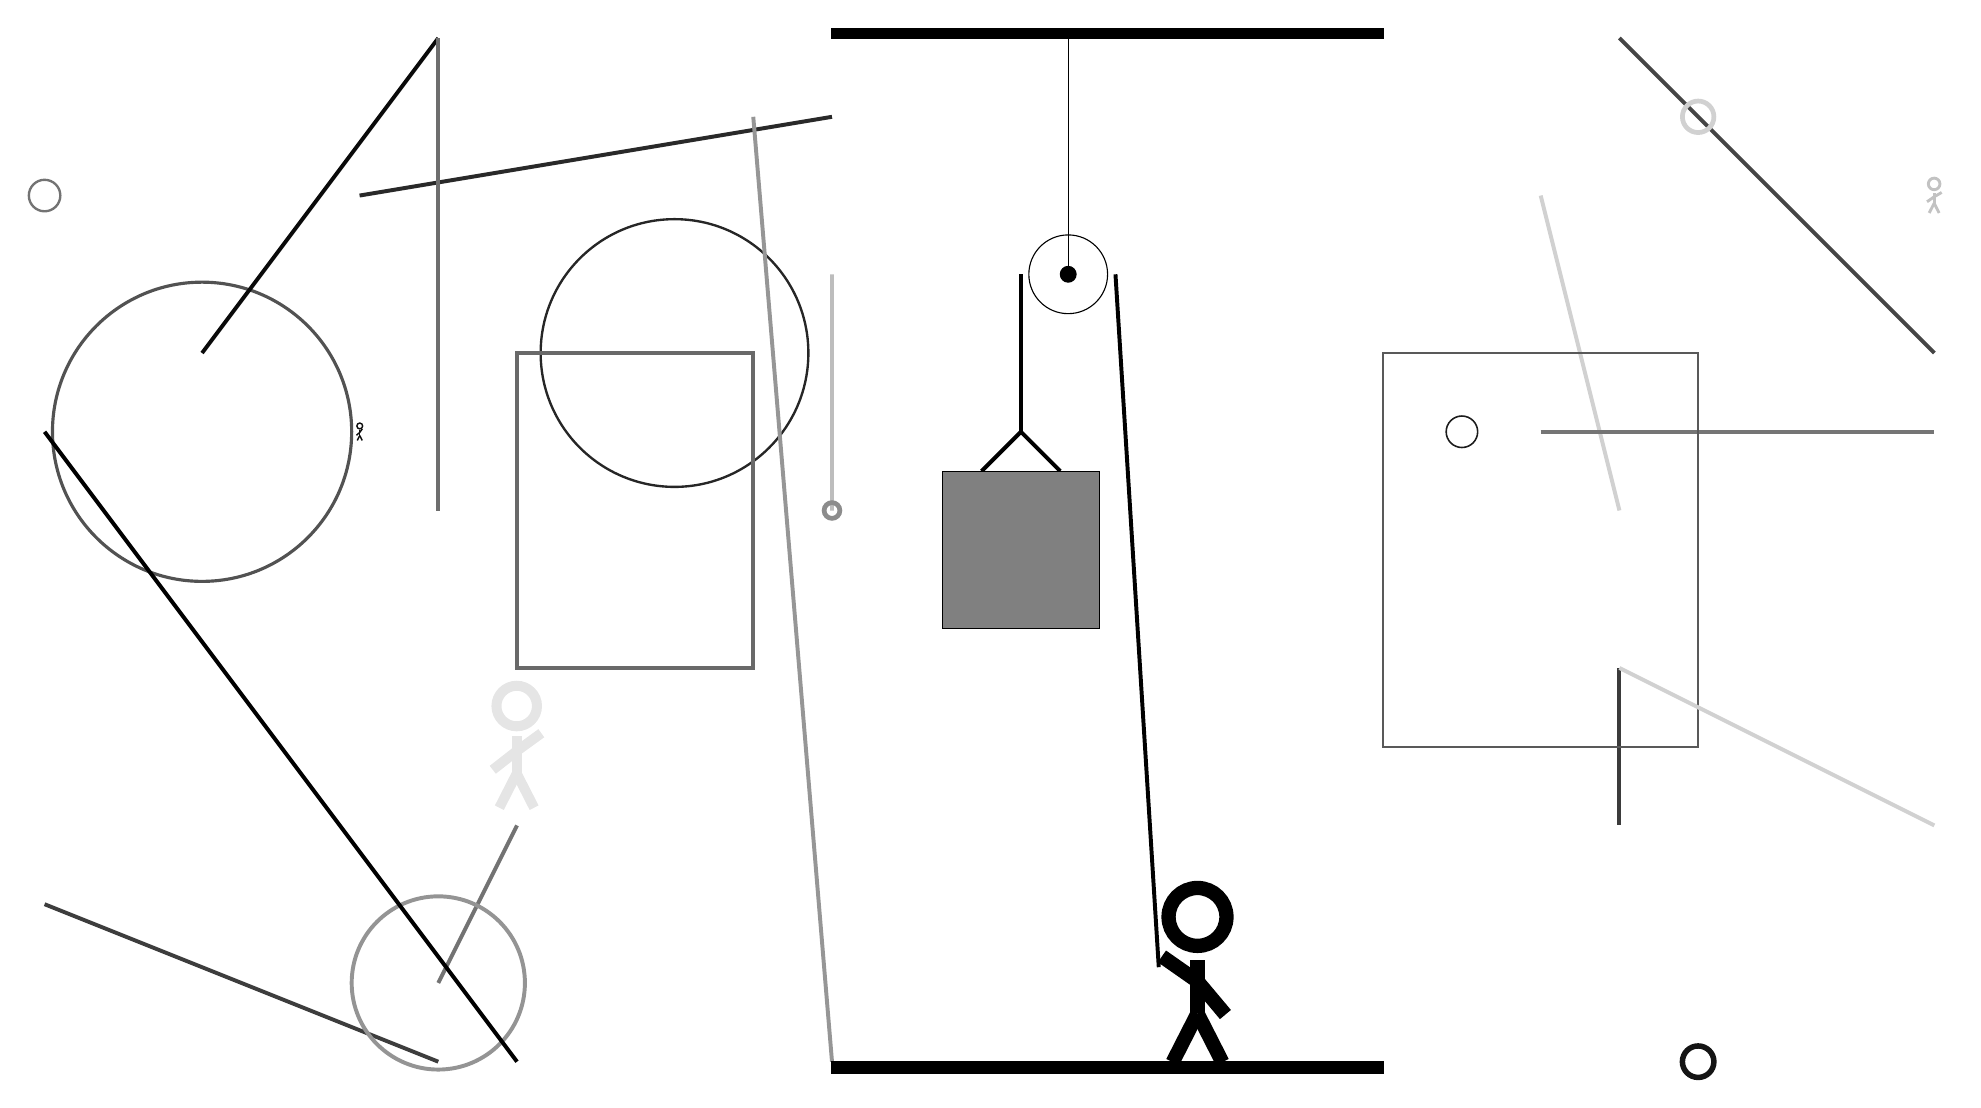
\begin{tikzpicture}
		%%%%% START %%%%%
		
		\draw[fill=black] (-2, 10) rectangle (5, 10.125);
		
		\draw[line width=0.5mm, color=black!84](-2, 9) -- (-8, 8);
		
		\node[line width=0.3mm, color=black!24] at (12, 8) {\Strichmaxerl[2][35][30]};
		\draw[line width=0.6mm, color=black!26] (-2, 4) rectangle (-2, 7);
		\draw[line width=0.5mm, color=black!76](-7, -3) -- (-12, -1);
		\draw[line width=0.5mm, color=black!77](8, 2) -- (8, 0);
		
		\draw[line width=0.5mm, color=black!18](8, 4) -- (7, 8);
		
		\draw [line width=0.3mm, color=black!85](-4, 6) circle (1.7);
		\draw [line width=0.4mm, color=black!68](-10, 5) circle (1.9);
		\node[line width=0.6mm, color=black!95] at (-8, 5) {\Strichmaxerl[1][41][54]};
		
		\draw[line width=0.5mm, color=black!54](7, 5) -- (12, 5);
		
		\node[line width=0.7mm, color=black!10] at (-6, 1) {\Strichmaxerl[7][38][36]};
		\draw [line width=0.3mm, color=black!55](-12, 8) circle (0.2);
		\draw[line width=0.5mm, color=black!55](-7, -2) -- (-6, 0);
		\draw [line width=0.6mm, color=black!45](-2, 4) circle (0.1);
		\draw [line width=0.5mm, color=black!42](-7, -2) circle (1.1);
		\draw[line width=0.3mm, color=black!65] (5, 6) rectangle (9, 1);
		\draw[line width=0.5mm, color=black!100](-6, -3) -- (-12, 5);
		
		\draw[line width=0.5mm, color=black!56](-6, 1) -- (-6, 1);
		\draw[line width=0.5mm, color=black!18](8, 2) -- (12, 0);
		\draw[line width=0.5mm, color=black!73](8, 10) -- (12, 6);
		\draw [line width=0.7mm, color=black!92](9, -3) circle (0.2);
		
		\draw [line width=0.2mm, color=black!89](6, 5) circle (0.2);
		\draw[line width=0.5mm, color=black!96](-7, 10) -- (-10, 6);
		\draw [line width=0.6mm, color=black!18](9, 9) circle (0.2);
		\draw[line width=0.5mm, color=black!59] (-3, 2) rectangle (-6, 6);
		
		\draw[line width=0.5mm, color=black!41](-2, -3) -- (-3, 9);
		
		\draw[line width=0.5mm, color=black!57](-7, 10) -- (-7, 4);
		
		\draw (1, 7) circle (0.5);
		\draw[fill=black] (1, 7) circle (0.1);
		\draw (1, 10) -- (1, 7);
		
		\draw[line width=0.5mm] (-0.1, 4.5) -- (0.4, 5.0) -- (0.9, 4.5);
		\draw[fill=black!50] (-0.6, 4.5) rectangle (1.4, 2.5);
		
		\draw[line width=0.5mm] (0.4, 7) -- (0.4, 5.0);
		\centerarc[line width=0.5mm](1, 7)(0:180:0.6);
		\draw[line width=0.5mm](1.6, 7) -- (2.15, -1.8);
		
		\node at (2.6, -1.9) {\Strichmaxerl[10][-35][-50]};
		
		\draw[fill=black] (-2, -3) rectangle (5, -3.15);
		
		%%%%% END %%%%%
	\end{tikzpicture}
\end{document}